\documentclass{article}
\usepackage[a4paper, margin=1in]{geometry}
\usepackage{amsmath}
\usepackage{graphicx}
\usepackage{amsfonts}
\usepackage{amssymb}

% Packages for drawing diagrams
\usepackage{tikz}
\usetikzlibrary{arrows.meta, positioning}

\title{Mastering the Cosmic Commute: A Guide to the Hohmann Orbit Transfer}
\author{}
\date{}

\begin{document}

\maketitle

The \textbf{Hohmann transfer orbit} is a fundamental and highly fuel-efficient maneuver used to move a spacecraft between two different circular orbits that are in the same plane. Conceived by German engineer Walter Hohmann in 1925, this elliptical path is a cornerstone of orbital mechanics, crucial for missions ranging from satellite deployment to interplanetary voyages.

\section*{Core Concepts: The Elliptical Bridge}

Imagine two circular highways around a central body, like the Earth. The Hohmann transfer is the elliptical on-ramp and off-ramp that allows a spacecraft to seamlessly move between them.

The maneuver relies on two brief engine burns, known as \textbf{impulsive burns}:
\begin{itemize}
    \item \textbf{First Burn ($\Delta v_1$):} Initiates the transfer by pushing the spacecraft into the elliptical orbit.
    \item \textbf{Second Burn ($\Delta v_2$):} Occurs upon arrival at the target orbit to circularize the path.
\end{itemize}

The transfer orbit itself is a carefully calculated ellipse that is \textbf{tangent} to both the initial and final circular orbits at two key points.

\subsection*{Apoapsis and Periapsis}

In any elliptical orbit, there are two points of significance:
\begin{itemize}
    \item \textbf{Apoapsis:} The point on the orbit \textit{farthest} from the central body. The "apo-" prefix means away or off.
    \item \textbf{Periapsis:} The point on the orbit \textit{closest} to the central body. The "peri-" prefix means near.
\end{itemize}

For a Hohmann transfer from an inner to an outer orbit, the first burn happens at the periapsis of the transfer ellipse, and the second burn occurs at its apoapsis. The reverse is true for an outer-to-inner transfer.

\begin{center}
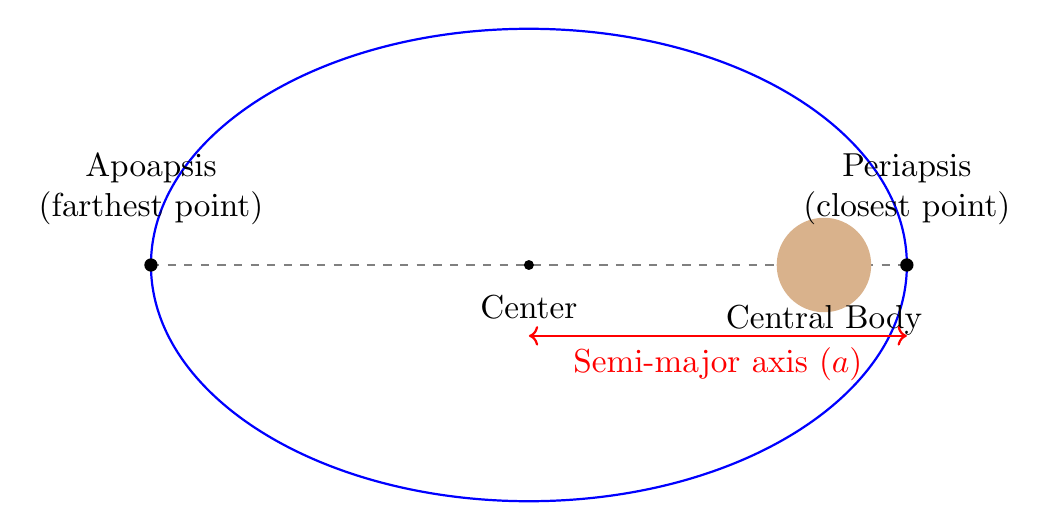
\begin{tikzpicture}[scale=1.2, every node/.style={transform shape}]
    % Define ellipse parameters
    \def\a{4} % Semi-major axis
    \def\b{2.5} % Semi-minor axis
    % Calculate focus distance c = sqrt(a^2 - b^2)
    \pgfmathsetmacro{\c}{sqrt(\a*\a - \b*\b)}

    % Draw the major axis line for reference
    \draw[dashed, gray] (-\a,0) -- (\a,0);
    
    % Draw the elliptical orbit path
    \draw[thick, blue] (0,0) ellipse (\a cm and \b cm);
    
    % Draw the central body at one focus
    \node[circle, fill=brown!60, minimum size=1cm, label={[label distance=-2mm]below:Central Body}] (F) at (\c,0) {};
    
    % Mark the center of the ellipse
    \fill (0,0) circle (1.5pt);
    \node[below=2mm] at (0,0) {Center};

    % Mark and label Periapsis (closest point to the focus F)
    \fill (\a,0) circle (2pt);
    \node[above=3mm, align=center] at (\a,0) {Periapsis \\ (closest point)};
    
    % Mark and label Apoapsis (farthest point from the focus F)
    \fill (-\a,0) circle (2pt);
    \node[above=3mm, align=center] at (-\a,0) {Apoapsis \\ (farthest point)};
    
    % Draw and label the semi-major axis 'a'
    \draw[<->, thick, red] (0, -0.75) -- (\a, -0.75);
    \node[below, red] at (\a/2, -0.75) {Semi-major axis ($a$)};
\end{tikzpicture}
\end{center}

\section*{The Mathematics of the Maneuver}

Our calculations hinge on the \textbf{vis-viva equation}, which is a powerful tool relating a spacecraft's speed to its position in orbit.

\subsection*{Understanding the Standard Gravitational Parameter ($\mu$)}

Before diving into the vis-viva equation, let's clarify a key term: the \textbf{standard gravitational parameter ($\mu$)}. It's a shorthand used by orbital mechanics experts to simplify calculations. Instead of plugging in two separate constants, we use their product:
\[ \mu = GM \]
Where:
\begin{itemize}
    \item \textbf{G} is the universal gravitational constant ($\approx 6.674 \times 10^{-11} \text{ N m}^2/\text{kg}^2$).
    \item \textbf{M} is the mass of the central body (e.g., the Earth).
\end{itemize}
For Earth, $\mu \approx 398,600 \text{ km}^3/\text{s}^2$. Using $\mu$ streamlines our orbital equations.

\subsection*{Derivation of the Vis-Viva Equation}

The vis-viva ("living force") equation comes directly from the \textbf{conservation of energy}. The total energy ($E$) of an orbiting body is the sum of its kinetic energy (KE) and its gravitational potential energy (GPE).
\[ E = KE + GPE = \frac{1}{2}mv^2 - \frac{GMm}{r} \]
The total energy of an elliptical orbit can also be expressed in terms of its semi-major axis ($a$):
\[ E = -\frac{GMm}{2a} \]
By setting these two expressions for energy equal to each other, we get:
\[ \frac{1}{2}mv^2 - \frac{GMm}{r} = -\frac{GMm}{2a} \]
Dividing by the spacecraft's mass, $m$, and substituting $\mu = GM$:
\begin{align*}
    \frac{1}{2}v^2 - \frac{\mu}{r} &= -\frac{\mu}{2a} \\
    v^2 &= \mu \left( \frac{2}{r} - \frac{1}{a} \right)
\end{align*}
This gives us the celebrated \textbf{vis-viva equation}:
\begin{equation}
    v = \sqrt{\mu \left( \frac{2}{r} - \frac{1}{a} \right)}
\end{equation}
For a \textbf{circular orbit}, the radius is constant ($r=a$), so the equation simplifies to:
\begin{equation}
    v_{circular} = \sqrt{\frac{\mu}{r}}
\end{equation}
The \textbf{semi-major axis of the Hohmann transfer orbit ($a_t$)} is the average of the radii of the initial ($r_1$) and final ($r_2$) orbits:
\begin{equation}
    a_t = \frac{r_1 + r_2}{2}
\end{equation}

\section*{Case Study 1: Inner to Outer Orbit Transfer}

Let's move a satellite from a low Earth orbit (LEO) to a higher geosynchronous orbit (GEO).
\begin{center}
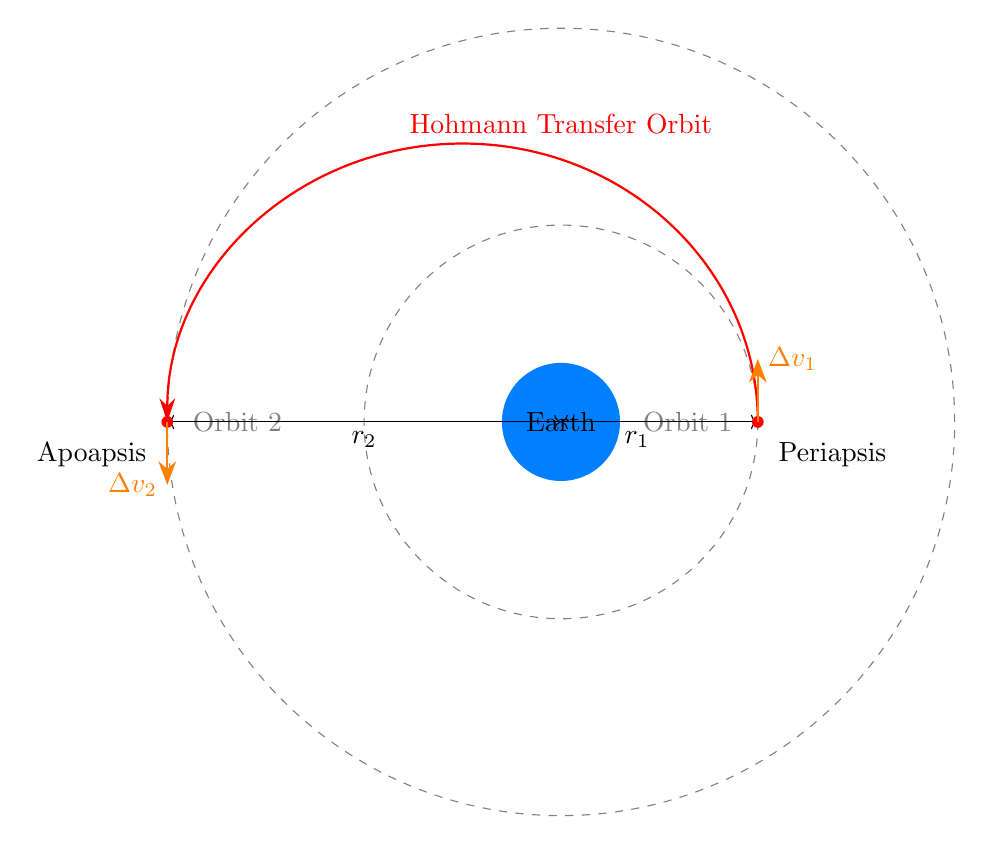
\begin{tikzpicture}[scale=1.0, every node/.style={transform shape}]
    % Radii
    \def\rOne{2.5}
    \def\rTwo{5}
    % Semi-major axis of transfer orbit
    \pgfmathsetmacro{\aT}{(\rOne+\rTwo)/2}
    % Center of transfer ellipse
    \pgfmathsetmacro{\cT}{\aT-\rOne}
    % Semi-minor axis of transfer orbit
    \pgfmathsetmacro{\bT}{sqrt(\aT*\aT - \cT*\cT)}

    % Draw central body (Earth)
    \node[circle, fill=blue!50!cyan, minimum size=1.5cm, label=center:Earth] (earth) at (0,0) {};

    % Draw initial inner circular orbit (Orbit 1)
    \draw[dashed, gray] (0,0) circle (\rOne cm);
    \node[left=2mm, gray] at (\rOne,0) {Orbit 1};

    % Draw final outer circular orbit (Orbit 2)
    \draw[dashed, gray] (0,0) circle (\rTwo cm);
    \node[right=2mm, gray] at (-\rTwo,0) {Orbit 2};

    % Draw Hohmann transfer orbit (half ellipse)
    \draw[thick, red, -{Stealth[length=3mm, width=2mm]}] (\rOne,0) arc (0:180:{\aT} and {\bT});
    \node[above, red] at (0, \bT) {Hohmann Transfer Orbit};
    
    % Label Radii
    \draw[<->] (0,0) -- node[midway, below left] {$r_1$} (\rOne,0);
    \draw[<->] (0,0) -- node[midway, below] {$r_2$} (-\rTwo,0);
    
    % Indicate First Burn (Prograde)
    \node[circle, fill=red, inner sep=1.5pt] at (\rOne,0) {};
    \draw[thick, orange, -{Stealth[length=3mm]}] (\rOne,0) -- ++(0,0.8) node[right] {$\Delta v_1$};
    \node[below right=2mm] at (\rOne,0) {Periapsis};

    % Indicate Second Burn (Prograde)
    \node[circle, fill=red, inner sep=1.5pt] at (-\rTwo,0) {};
    \draw[thick, orange, -{Stealth[length=3mm]}] (-\rTwo,0) -- ++(0,-0.8) node[left] {$\Delta v_2$};
    \node[below left=2mm] at (-\rTwo,0) {Apoapsis};
\end{tikzpicture}
\end{center}

\subsection*{1. First Velocity Adjustment ($\Delta v_1$)}
At the periapsis ($r_1$), we perform a prograde (forward) burn to increase speed and enter the elliptical transfer orbit.
\begin{itemize}
    \item \textbf{Initial Velocity ($v_1$):} $v_1 = \sqrt{\frac{\mu}{r_1}}$
    \item \textbf{Velocity at Periapsis ($v_{p}$):} $v_{p} = \sqrt{\mu \left( \frac{2}{r_1} - \frac{1}{a_t} \right)}$
    \item \textbf{The First Burn:} $\Delta v_1 = v_{p} - v_1$
\end{itemize}

\subsection*{2. Second Velocity Adjustment ($\Delta v_2$)}
Upon reaching the apoapsis ($r_2$), we perform another prograde burn to increase speed and circularize the orbit at GEO.
\begin{itemize}
    \item \textbf{Velocity at Apoapsis ($v_{a}$):} $v_{a} = \sqrt{\mu \left( \frac{2}{r_2} - \frac{1}{a_t} \right)}$
    \item \textbf{Final Velocity ($v_2$):} $v_2 = \sqrt{\frac{\mu}{r_2}}$
    \item \textbf{The Second Burn:} $\Delta v_2 = v_2 - v_{a}$
\end{itemize}
\textbf{Example:} A satellite in a 300 km altitude orbit moves to a 35,786 km altitude orbit. With $r_1 = 6671$ km and $r_2 = 42157$ km, the total change in velocity, \textbf{Total $\Delta v$}, is $\Delta v_1 + \Delta v_2 \approx 3.88 \text{ km/s}$.

\section*{Case Study 2: Outer to Inner Orbit Transfer}
Now, let's bring a spacecraft from a higher orbit to a lower one. This involves decreasing speed.
\begin{center}
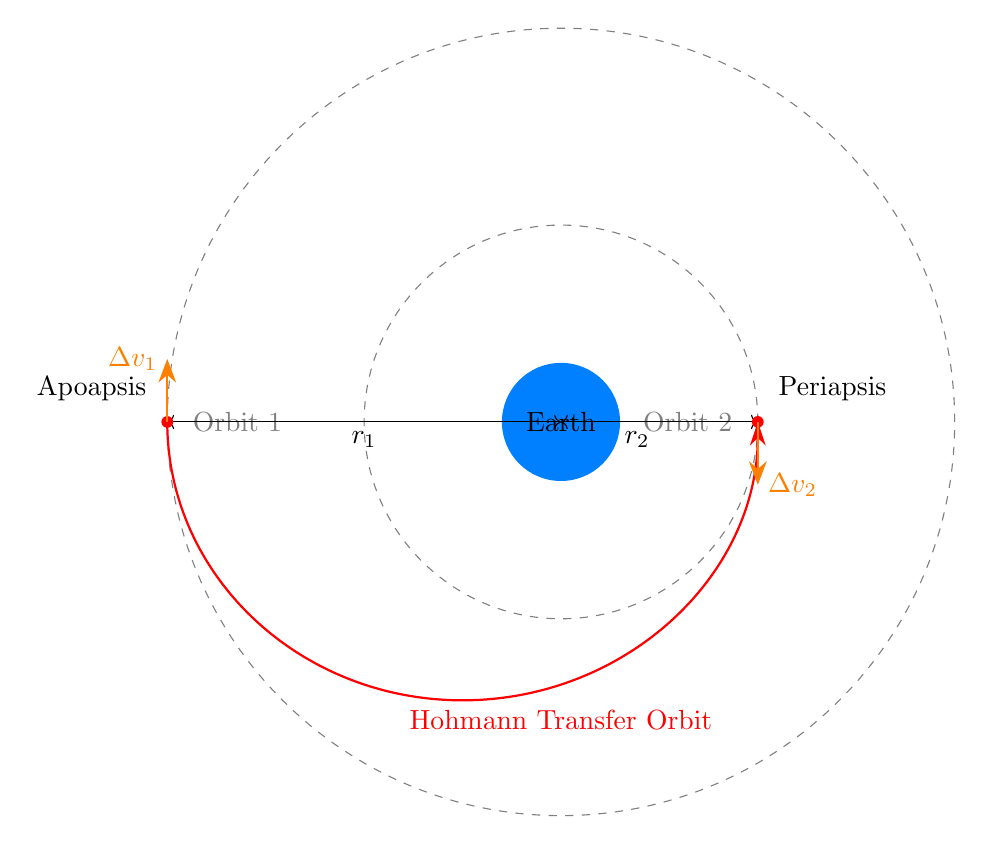
\begin{tikzpicture}[scale=1.0, every node/.style={transform shape}]
    % Radii
    \def\rOne{5} % Starting orbit
    \def\rTwo{2.5} % Final orbit
    % Semi-major axis of transfer orbit
    \pgfmathsetmacro{\aT}{(\rOne+\rTwo)/2}
    % Center of transfer ellipse
    \pgfmathsetmacro{\cT}{\aT-\rTwo}
    % Semi-minor axis of transfer orbit
    \pgfmathsetmacro{\bT}{sqrt(\aT*\aT - \cT*\cT)}

    % Draw central body (Earth)
    \node[circle, fill=blue!50!cyan, minimum size=1.5cm, label=center:Earth] (earth) at (0,0) {};

    % Draw initial outer circular orbit (Orbit 1)
    \draw[dashed, gray] (0,0) circle (\rOne cm);
    \node[right=2mm, gray] at (-\rOne,0) {Orbit 1};

    % Draw final inner circular orbit (Orbit 2)
    \draw[dashed, gray] (0,0) circle (\rTwo cm);
    \node[left=2mm, gray] at (\rTwo,0) {Orbit 2};

    % Draw Hohmann transfer orbit (half ellipse)
    \draw[thick, red, -{Stealth[length=3mm, width=2mm]}] (-\rOne,0) arc (180:360:{\aT} and {\bT});
    \node[below, red] at (0, -\bT) {Hohmann Transfer Orbit};
    
    % Label Radii
    \draw[<->] (0,0) -- node[midway, below] {$r_1$} (-\rOne,0);
    \draw[<->] (0,0) -- node[midway, below left] {$r_2$} (\rTwo,0);
    
    % Indicate First Burn (Retrograde)
    \node[circle, fill=red, inner sep=1.5pt] at (-\rOne,0) {};
    \draw[thick, orange, -{Stealth[length=3mm]}] (-\rOne,0) -- ++(0,0.8) node[left] {$\Delta v_1$};
    \node[above left=2mm] at (-\rOne,0) {Apoapsis};

    % Indicate Second Burn (Retrograde) - FINAL CORRECTION
    \node[circle, fill=red, inner sep=1.5pt] at (\rTwo,0) {};
    \draw[thick, orange, -{Stealth[length=3mm]}] (\rTwo,0) -- ++(0,-0.8) node[right] {$\Delta v_2$};
    \node[above right=2mm] at (\rTwo,0) {Periapsis};
\end{tikzpicture}
\end{center}

\subsection*{1. First Velocity Adjustment ($\Delta v_1$)}
At the apoapsis ($r_1$), we perform a retrograde (braking) burn to decrease speed and enter the transfer ellipse.
\begin{itemize}
    \item \textbf{Initial Velocity ($v_1$):} $v_1 = \sqrt{\frac{\mu}{r_1}}$
    \item \textbf{Velocity at Apoapsis ($v_{a}$):} $v_{a} = \sqrt{\mu \left( \frac{2}{r_1} - \frac{1}{a_t} \right)}$
    \item \textbf{The First Burn:} $\Delta v_1 = v_1 - v_{a}$
\end{itemize}

\subsection*{2. Second Velocity Adjustment ($\Delta v_2$)}
Upon reaching the periapsis ($r_2$), we perform another retrograde burn to slow down further and circularize into the lower orbit.
\begin{itemize}
    \item \textbf{Velocity at Periapsis ($v_{p}$):} $v_{p} = \sqrt{\mu \left( \frac{2}{r_2} - \frac{1}{a_t} \right)}$
    \item \textbf{Final Velocity ($v_2$):} $v_2 = \sqrt{\frac{\mu}{r_2}}$
    \item \textbf{The Second Burn:} $\Delta v_2 = v_{p} - v_2$
\end{itemize}
\textbf{Example:} A spacecraft moves from a 20,000 km radius orbit to a 10,000 km radius orbit. With $r_1 = 20000$ km and $r_2 = 10000$ km, the \textbf{Total $\Delta v$} required is $\Delta v_1 + \Delta v_2 \approx 1.79 \text{ km/s}$.

\section*{Timing is Everything: Calculating the Transfer Time}
The time it takes to complete a Hohmann transfer is exactly \textbf{half the orbital period of the transfer ellipse}. We can calculate this using Kepler's Third Law. The period of an orbit ($T$) is given by:
\[ T = 2\pi \sqrt{\frac{a^3}{\mu}} \]
For the Hohmann transfer, the time of flight ($t_{transfer}$) is:
\begin{equation}
    t_{transfer} = \frac{1}{2} T_t = \pi \sqrt{\frac{a_t^3}{\mu}}
\end{equation}
For our LEO to GEO example ($a_t = 24414$ km):
\[ t_{transfer} = \pi \sqrt{\frac{24414^3}{398600}} \approx 19045 \text{ seconds} \]
This is approximately \textbf{5.29 hours}.

\end{document}